%location/filename: tex/ch1.tex
%author: Anders Østevik
%Last edited: 26.05.2016
%#######--Chapter 1--#######
%Content:
%	Introduction
%	

\documentclass[main.tex]{subfiles}

\begin{document}

\chapter{Introduction}

\section{LHC}

The \gls{lhc} is the largest and most powerful particle collider in the world. It was built by the European Organization for Nuclear Research (CERN) \cite{cernweb} between 1998 and 2008, and had its first start-up on 10 September 2008. This massive machine lies 175 metres deep beneath the France–Switzerland border near Geneva, Switzerland; and consists of a $27~\kilo\meter$ long circular tunnel of superconductor magnets with additional accelerating structures. Its basic operation is to accelerate particles (protons and heavy ions, e.g. Pb) to near the speed of light in opposite directions and collide them. The particles are accelerated along two parallel beam lines running through the superconductor magnets, and collided at four locations were experiments like ATLAS\cite{atlasweb}, ALICE\cite{aliceweb}, CMS\cite{cmsweb} and LHCb\cite{lhcbweb} take place. As of 20 May 2015, the \gls{lhc} can achieve beam energies up to $13~\tera e\volt$, or $6.5~\tera e\volt$ per beam.

\section{SLHC}

The future upgrade of the \sebo{\gls{lhc}} accelerator, the \gls{slhc}, has its goal of increasing the beam luminosity by ten times. This will lead to a corresponding growth of the amount of data to be treated by the data acquisition systems, and an increase in radiation. This will thus require high rate data links and \glspl{asic} capable of tolerating high doses of radiation.

To address these needs, the \gls{gbt} architecture and transmission protocol was developed to provide a high radiation tolerant, high speed, optical transmission line capable with a simultaneous transfer of readout data, timing and trigger signals in addition to slow control and monitoring data.

\section{GBT system}
The \gls{gbt} system can be described in two parts: The on-detector part, and the off-detector part of the system. The below sections gives a brief description of these:

\subsection{On-detector}
The on-detector part consists of radiation hard GBT \acrshort{asic}s that will provide interface and data transmission to the detectors and will thus be located in the radioactive zone. These \glspl{asic} are used to implement bi-directional multipurpose $4.8~\giga\bit\per\second$ optical links for the high-energy physics experiments.

\subsubsection{GBTx}
The GBTx \gls{asic} is a serializer-de-serializer chip responsible for the high speed bi-directional optical link. It has a bandwidth of $3.2 - 4.8~\giga\bit\per\second$, and combines three data paths for Trigger and Timing Control (TTC), Data Acquisition (DAQ) and Slow Control (SC) information in one physical link; using two optical fibers. The GBTx encodes and decodes this information into what is known as the GBT-Frame, and provides interface to the front end electronics embedded in the detectors. \cite{gbtxman11}

\subsubsection{GBT frame formats}
 The GBTx transmits a 120-bit frame every $25~\nano\second$ ($40~\mega\hertz$), which is triggered by LCH bunch crossings. The GBTx supports three different encoding modes: "GBT-Frame", "8B/10B" and "Wide-Bus" mode. Figure \ref{fig:gbtframe} illustrates the "GBT-Frame" mode: The Header (H) field is a 4-bit field transmitted at the beginning of each frame, used to synchronize the data stream at the frame level. The header field can be set to "idle" (0110) or "data" (0101). The Slow Control (SC) field is a 4-bit field dedicated for routine and control operations that do not require precise timing. The Data field is a 80-bit field reserved for generic transmission of data with a corresponding bandwidth of $3.2~\giga\bit\per\second$. The remaining field reserves 32 bits for Forward Error Correction (FEC). FEC involves using Reed-Solomon encoding capable of correcting up to 16 concecutive corrupted bits. To achieve DC-balancing, a self-synchronizing scrambler distributes the 0's and 1's in the data stream.

The "8B/10B" and "Wide-Bus" mode share simularities with the "GBT-Frame" mode, but favors data width over lesser grades of error correction (the "Wide-Bus" has none). Both modes are only available in the transmitter part of the GBTx, but requires less resources from the \gls{fpga} (receiving end) than the "GBT-Frame". The "8B/10B" does not require scrambling because it is in itself DC-balanced. \cite{gbtxman11}. These two modes are not yet available in the GBT FPGA example design.

Both GBTx encoding and decoding operations can be done within a single clock cycle at $40~\mega\hertz$. 
 
\begin{figure} % H(strictly put HERE > h!)
% h(here), !(force), t(top), b(bottom), p(on extra page)
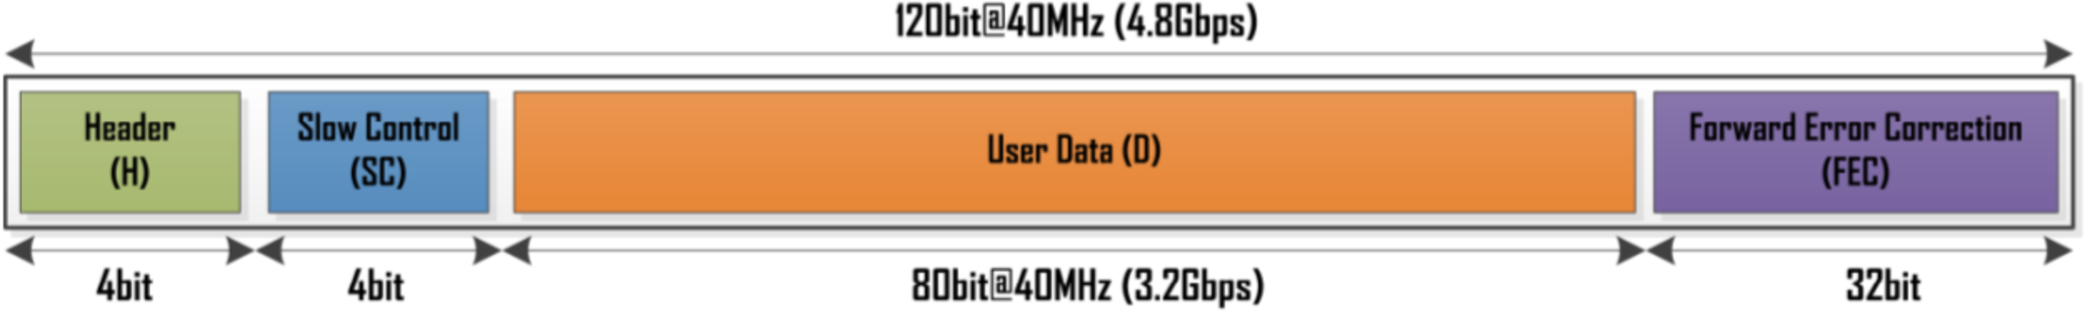
\includegraphics[width=\linewidth]{../img/gbtframe}  \\[0.1 cm]
\caption{The GBT-Frame format. \cite[Figure 4]{gbt_fpga}.}
\label{fig:gbtframe}
\end{figure}

\subsubsection{GBT-SCA}

The \gls{sca} \gls{asic} is the part of the \gls{gbt} chipset which distributes control and monitoring signals to the front-end electronics embedded in the detectors. It connects to the GBTx through a dedicated $80~\mega\bit\per\second$ e-link and provides a number of user interface options for the front-end detectors, which includes: SPI, \acrshort{iic}, JTAG and a number of \acrshort{gpio}s \cite{gbtsca15}. \\

\noindent
All chips has been implemented using a commercial $130~\nano\meter$ process because of benefits regarding inherent resistance to ionising radiation \cite{gbtpro10}.

\subsection{Off-detector}
The off-detector part is located in the counting room and consists of a \gls{cru}, that will provide an interface between the detector \acrshort{asic}s and an online computer farm, with the GBTx as the middle joint. The \gls{cru} consists of \gls{cots} components, mainly an \gls{fpga}, and will through optical links receive the data from the radiation detector.

\subsubsection{FPGA - Cyclone V GT} \label{sec:cyclone}

Altera's Cyclone V GT \gls{fpga} board was chosen for use in this thesis. It was chosen mainly because of the on-board transceivers that are capable of reaching speeds that surpass the requirements of the \gls{gbt}-\gls{fpga} \gls{mgt}, i.e $4.8~\giga\bit\per\second$; "GT" indicates that the \gls{fpga} has transceivers that support speeds up to $6~\giga\bit\per\second$ \cite{altera_cvoverview15}.\\
Originally, a Terasic Cyclone V GX development board was handed for use with this thesis. The Terasic board has advantages over the Cyclone V GT board in terms of communication with the outside world, such as on-board Usb-to-Uart (more on this  in chapter \ref{chap:sercom}). However, it was discovered that the transceivers on the Terasic board were not fast enough for the \gls{gbt} \gls{mgt}; maximum supported transceiver speed is only $3.125~\giga\bit\per\second$ \cite{altera_cvoverview15}. Because of this, the more powerful Cyclone V GT \gls{fpga} development board was ordered from the Altera web-pages, replacing the Terasic.

\section{Versatile Link Demo Board}

The \gls{vldb} is the evaluation kit for the radiation hard optical link. It includes the main elements of the GBT Link, the radiation hard \glspl{asic}; GBTx, GBT-SCA and the VTRx/VTTx, in addition to radiation hard DC/DC converters. The \gls{vldb} has 20 e-links reachable through \gls{hdmi} connectors that connects to the front-end electronics, and a fiber-optic link that connects to the off-detector \gls{fpga}.\\

\section{E-Links}
An E-link is an electrical interface suitable for transmission
Each E-link has three differential signal lines: a clock line (dClk+/dClk-), a downlink output (dOut+/dOut-) and a uplink input (dIn+/dIn-).


\begin{figure} % H(strictly put HERE > h!)
% h(here), !(force), t(top), b(bottom), p(on extra page)
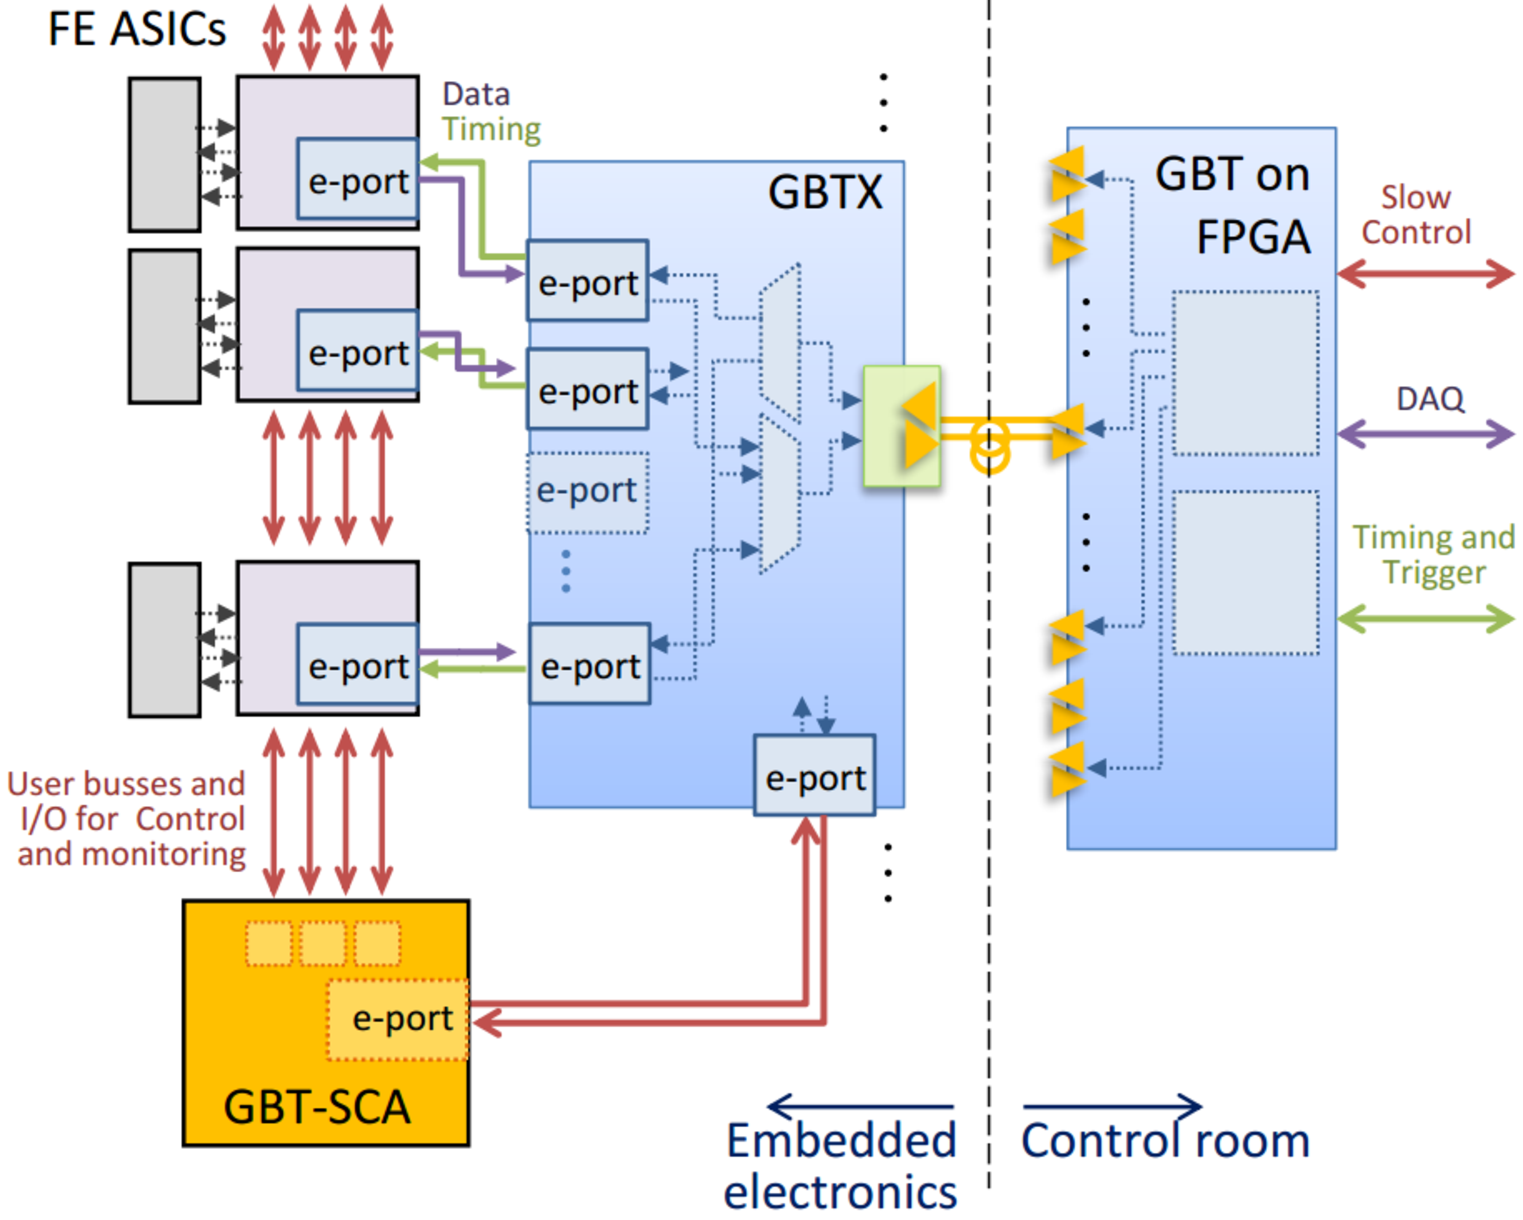
\includegraphics[width=0.7\linewidth]{../img/gbtsys}  \\[0.1 cm]
\caption{The GBT-link in its entirety. The on-detector consists of custom made \glspl{asic} with an optical link connecting the off-detector \gls{fpga} with the GBT-FPGA implemented. \cite[Figure 1]{gbtscapres14}.}
\label{fig:gbtsys}
\end{figure}

\section{Primary objective}
This thesis has its focus on the design of a \gls{cru} control interface software, and also a physical connection between the \gls{cru} and the \gls{vldb} card, where the radiation hard \gls{asic}, the \gls{gbt}x, is located. The control interface was developed with the goal of one day replacing the Quartus-bound \gls{issp}, which is used today to manipulate the \gls{gbt} control-signals; and instead introduce a cross-platform, open-source solution. 

\section{Outline}

%\todo{General:\\PLLs\\CPRI?\\}

\chapter{Cyclone V Transceiver Technology}

To be able to send serial data in the gigahertz domain, a high-speed transceiver is required. The Cyclone V GT-series \glspl{fpga} supports a number of transceiver technologies through the \gls{hsmc} physical interface that can reach speeds up to $6.144\ \giga\bit\per\second$. This section gives a general description of some of these protocols.

\subsection{Differential Signals} \label{subsec:diffsig}

Common for all protocols described is the fact that the signals are treated differentially. 

While a single ended signal involves one conductor between the transmitter and receiver, with the signal swinging from a given voltage to ground; differential signals involves a conductor pair with two signals that are identical, but with opposite polarity. The pair would ideally have equal path lenghts in order to have zero return currents, avoiding problems like \textit{EMI}. In addition, placing the signals as close as possible to one another will give benefits in terms of common noise rejection \cite{douglas01}.\\

When done correctly, differential signals have advantages over single ended signals such as effective isolation from power systems, minimized crosstalk and noise immunity through common-mode noise rejection. It also improves S/N ratio and effectively doubles the signal level at the output $(+v - (-v) = 2v)$, which makes it especially useful in low signal applications. The disadvantage comes in an increase in pin count and space required, since differential signals consists of two wires instead of one \cite{douglas01}.

\subsection{Low-Voltage Differential Signaling}

\gls{lvds} is said to be the most commonly used differential interface. The interface offers a low power consumption with a voltage swing of $350\ \milli\volt$ and good noise immunity. LVDS can deliver data rates up to $3.125\ \giga\bit\per\second$ \cite{ti08lvds}.\\

The Cyclone V GT board has 17 \gls{lvds} channels available on the \gls{hsmc} port A connector. The channels have the ability to transmit and receive data at a rate up to $840\ \mega\bit\per\second$, with support for serialization and deserialization through internal logic. \cite{altera_cvoverview15}

\subsection{Current-Mode Logic}

For data rates that exceeds $3.125\ \giga\bit\per\second$, \gls{cml} signaling is preferred. This is due to the fact that certain communication standards such as \acrshort{pcie}, \acrshort{sata} and \acrshort{hdmi}, shares consistency with CML in signal amplitude and reference to $Vcc$. CML can reach a data rate in excess of $10\ \giga\bit\per\second$, but has a higher power consumption than \gls{lvds}, with a voltage swing of approximately $800\ \milli\volt$ \cite{ti08lvds}.\\

The Cyclone V GT board has 4 Pseudo-\gls{cml} (PCML) channels available on both port A and B \gls{hsmc} connectors. The channels have the ability to transmit and receive data at a rate up to $5.0\ \giga\bit\per\second$, just over the $4.8\ \giga\bit\per\second$ range required by the \gls{gbt} \gls{mgt}. \cite{altera_cyclonekit}


%\subsection{CPRI}

%\subsection{Phase-Locked Loops}

%A \gls{pll} is a device


\chapter{The Gigabit Transceiver} \label{chap:gbt}

\todo{History, mgt, Short about the electronic components, gbt-sca, gbtx}

\section{Encoding modes}

The "GBT-Frame" mode, which is Reed-Solomon Based; the "8b10b" mode; and the "Wide-Bus" mode which is without encoding.

\section{GBT-FPGA Core}
The following sections describe the different components that makes up the GBT-FPGA Core. The information was obtained by reading the GBT-FPGA User Guide \cite{gbt_fpga}.

\subsection{GBT Bank}
The GBT Bank is defined as the top module of the \gls{gbt}-\gls{fpga} Core. It integrates up to four GBT Links and contains the ports required to operate the GBT Links.

\subsection{GBT Link}
The \gls{gbt} Link is the actual channel of the link. It is composed of three components: GBT Tx, GBT Rx, and the \gls{mgt}. The following subsections gives a brief description of these components.

\subsubsection{GBT Tx}

The \gls{gbt} Tx component is responsible for scrambling and encoding data before transmitting it through the \gls{mgt}.

\subsubsection{GBT Rx}

The \gls{gbt} Rx component is responsible for receiving, decoding and de-scrambling the data through the \gls{mgt}.

\subsubsection{Multi-Gigabit Transceiver}
The \gls{mgt} is responsible for the transmitting, receiving, serialization and de-serialization of the \gls{gbt} data. It is divided into a transmitter and a receiver part.\\ The transmitter contains a \gls{piso} with two input clocks; one for parallel data and one for serial data. It shifts in $40~\bit$ words from the GBT Tx with a reference clock of $120~\mega\hertz$, serializes the data and sends it out with the help of a dedicated Tx \gls{pll} that generates a serial clock of $2400 \mega\hertz$.\\ The receiver contains a \gls{cdr} block, a \gls{sipo}, a RXRECCLK Phase Aligner block and a Barrel-shifter. 

%\gls{cpri}


%\begin{align}
%	 b_1 &= s_{11}a_1 + s_{12}a_2 \\
%	 s_{21}a_1 + s_{22}a_2 &= b_2
%\end{align}


\end{document}

